\section{Approach Overview}
\label{overview:sec}

{\tool} has two main processes: training and predicting.

\subsection{Training Process}

Figure~\ref{overview-training} displays the general architecture of
{\tool}'s training process. The input of the training process is the
source code of the buggy method and one buggy statement. If a method
has multiple buggy statements, we treat one buggy statement and that
enclosing method at a time as a training instance. The output includes
the trained tree-based context learning model (\code{CCL} model to
learn the surrounding code context) and the trained tree-based code
transformation learning model (\code{CTL} model to learn the
bug-fixing code transformation) with their parameters. The training
process has two main steps:

\begin{figure}[t]
	\centering
	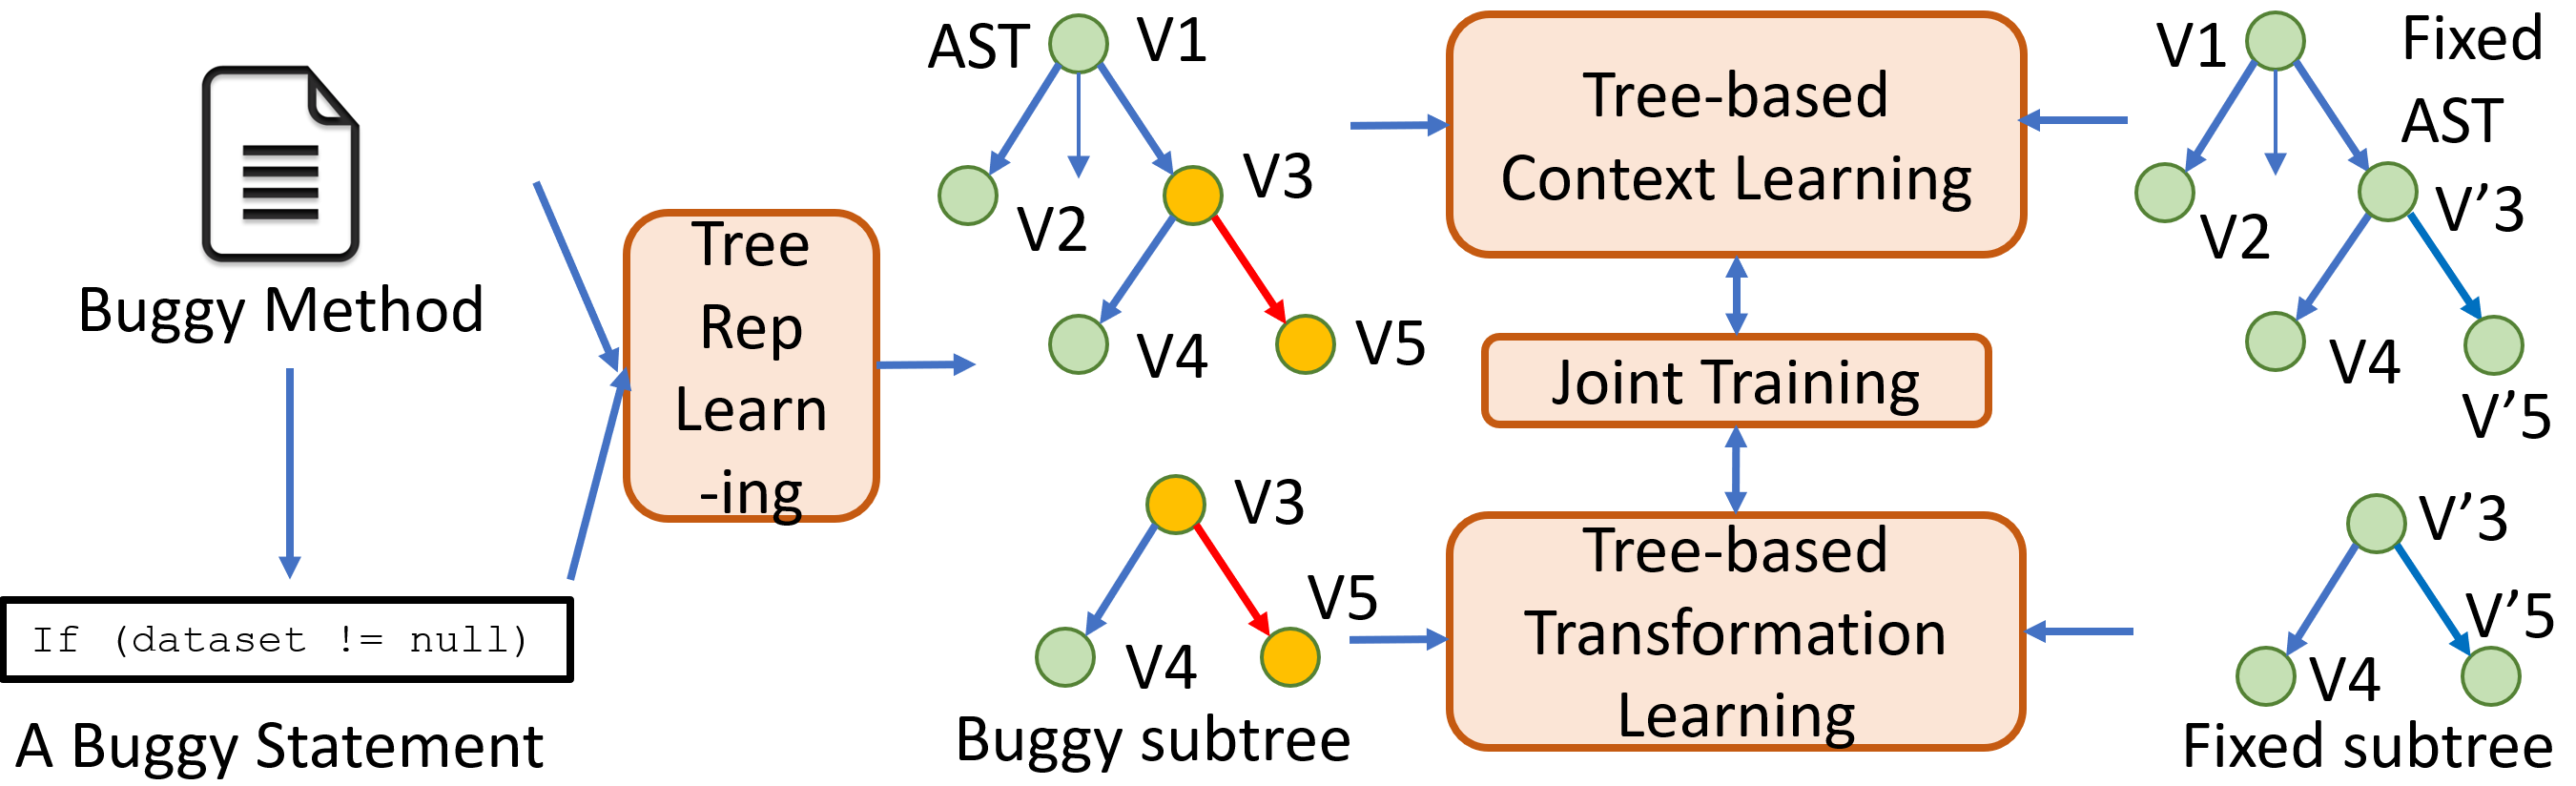
\includegraphics[width=3.4in]{graphs/overview-training.png}
	\caption{{\tool}: Training}
	\label{overview-training}
\end{figure}

\noindent 



\begin{figure}[t]
	\centering
	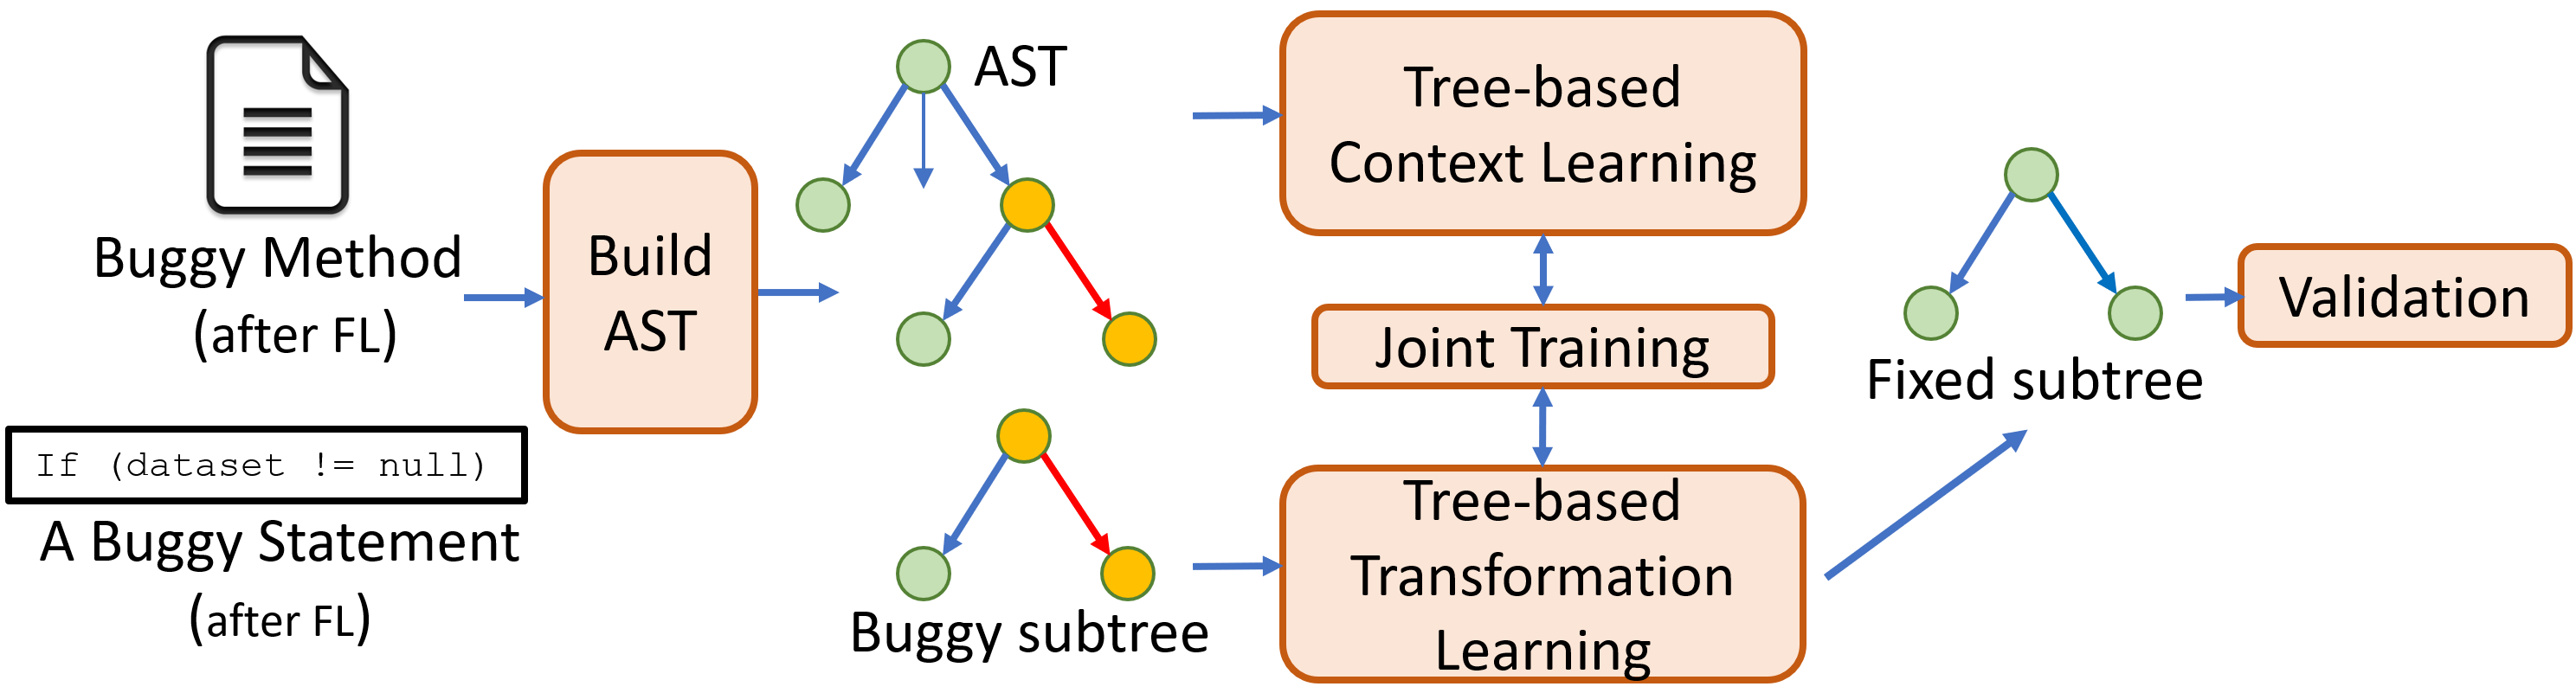
\includegraphics[width=3.4in]{graphs/overview-predict.png}
	\caption{{\tool}: Fixing}
	\label{overview-fixing}
\end{figure}

